% Options for packages loaded elsewhere
\PassOptionsToPackage{unicode}{hyperref}
\PassOptionsToPackage{hyphens}{url}
%
\documentclass[
  ignorenonframetext,
  aspectratio=169,
]{beamer}
\usepackage{pgfpages}
\setbeamertemplate{caption}[numbered]
\setbeamertemplate{caption label separator}{: }
\setbeamercolor{caption name}{fg=normal text.fg}
\beamertemplatenavigationsymbolsframe
% Prevent slide breaks in the middle of a paragraph
\widowpenalties 1 10000
\raggedbottom
\setbeamertemplate{part page}{
  \centering
  \begin{beamercolorbox}[sep=16pt,center]{part title}
    \usebeamerfont{part title}\insertpart\par
  \end{beamercolorbox}
}
\setbeamertemplate{section page}{
  \centering
  \begin{beamercolorbox}[sep=12pt,center]{part title}
    \usebeamerfont{section title}\insertsection\par
  \end{beamercolorbox}
}
\setbeamertemplate{subsection page}{
  \centering
  \begin{beamercolorbox}[sep=8pt,center]{part title}
    \usebeamerfont{subsection title}\insertsubsection\par
  \end{beamercolorbox}
}
\AtBeginPart{
  \frame{\partpage}
}
\AtBeginSection{
  \ifbibliography
  \else
    \frame{\sectionpage}
  \fi
}
\AtBeginSubsection{
  \frame{\subsectionpage}
}
\usepackage{lmodern}
\usepackage{amssymb,amsmath}
\usepackage{ifxetex,ifluatex}
\ifnum 0\ifxetex 1\fi\ifluatex 1\fi=0 % if pdftex
  \usepackage[T1]{fontenc}
  \usepackage[utf8]{inputenc}
  \usepackage{textcomp} % provide euro and other symbols
\else % if luatex or xetex
  \usepackage{unicode-math}
  \defaultfontfeatures{Scale=MatchLowercase}
  \defaultfontfeatures[\rmfamily]{Ligatures=TeX,Scale=1}
\fi
\usetheme[]{Copenhagen}
% Use upquote if available, for straight quotes in verbatim environments
\IfFileExists{upquote.sty}{\usepackage{upquote}}{}
\IfFileExists{microtype.sty}{% use microtype if available
  \usepackage[]{microtype}
  \UseMicrotypeSet[protrusion]{basicmath} % disable protrusion for tt fonts
}{}
\makeatletter
\@ifundefined{KOMAClassName}{% if non-KOMA class
  \IfFileExists{parskip.sty}{%
    \usepackage{parskip}
  }{% else
    \setlength{\parindent}{0pt}
    \setlength{\parskip}{6pt plus 2pt minus 1pt}}
}{% if KOMA class
  \KOMAoptions{parskip=half}}
\makeatother
\usepackage{xcolor}
\IfFileExists{xurl.sty}{\usepackage{xurl}}{} % add URL line breaks if available
\IfFileExists{bookmark.sty}{\usepackage{bookmark}}{\usepackage{hyperref}}
\hypersetup{
  pdftitle={Presentation Title},
  pdfauthor={Kevin Ernst},
  pdfsubject={A presentation about presentations with Markdown + Pandoc
+ Beamer},
  hidelinks,
  pdfcreator={LaTeX via pandoc}}
\urlstyle{same} % disable monospaced font for URLs
\newif\ifbibliography
\usepackage{graphicx}
\makeatletter
\def\maxwidth{\ifdim\Gin@nat@width>\linewidth\linewidth\else\Gin@nat@width\fi}
\def\maxheight{\ifdim\Gin@nat@height>\textheight\textheight\else\Gin@nat@height\fi}
\makeatother
% Scale images if necessary, so that they will not overflow the page
% margins by default, and it is still possible to overwrite the defaults
% using explicit options in \includegraphics[width, height, ...]{}
\setkeys{Gin}{width=\maxwidth,height=\maxheight,keepaspectratio}
% Set default figure placement to htbp
\makeatletter
\def\fps@figure{htbp}
\makeatother
\setlength{\emergencystretch}{3em} % prevent overfull lines
\providecommand{\tightlist}{%
  \setlength{\itemsep}{0pt}\setlength{\parskip}{0pt}}
\setcounter{secnumdepth}{-\maxdimen} % remove section numbering

\title{Presentation Title}
\subtitle{A presentation on presentations}
\author{Kevin Ernst}
\date{2021-08-22}
\institute{Weirauch Lab}

\begin{document}
\frame{\titlepage}

\hypertarget{section-one-title}{%
\section{Section One Title}\label{section-one-title}}

\hypertarget{intro-slide-title}{%
\subsection{Intro slide title}\label{intro-slide-title}}

\begin{frame}{Intro slide title}
A presentation about presentations.
\end{frame}

\hypertarget{slide-one}{%
\subsection{Slide one}\label{slide-one}}

\begin{frame}{Slide one}
\begin{itemize}[<+->]
\tightlist
\item
  point one
\item
  point two
\end{itemize}
\end{frame}

\hypertarget{slide-two}{%
\subsection{Slide two}\label{slide-two}}

\begin{frame}{Slide two}
This will not reveal incrementally, because it's in a blockquote.

\begin{itemize}
\tightlist
\item
  point one
\item
  point two
\end{itemize}
\end{frame}

\hypertarget{slide-with-a-pause}{%
\subsection{Slide with a pause}\label{slide-with-a-pause}}

\begin{frame}{Slide with a pause}
\framesubtitle{Look Ma, a subtitle!}

content before the pause

\pause
\end{frame}

\hypertarget{content-after-the-pause}{%
\subsubsection{content after the pause}\label{content-after-the-pause}}

\begin{frame}{content after the pause}
\begin{itemize}[<+->]
\tightlist
\item
  with
\item
  bullets
\end{itemize}
\end{frame}

\hypertarget{section-two}{%
\section{Section Two}\label{section-two}}

\hypertarget{two-a}{%
\subsection{Two-A}\label{two-a}}

\begin{frame}{Two-A}
\begin{columns}[T]
\begin{column}{0.48\textwidth}
\begin{itemize}[<+->]
\tightlist
\item
  it's a column!
\end{itemize}
\end{column}

\begin{column}{0.48\textwidth}
\begin{itemize}[<+->]
\tightlist
\item
  look, another one!
\end{itemize}
\end{column}
\end{columns}
\end{frame}

\hypertarget{section-three-title}{%
\section{Section Three Title}\label{section-three-title}}

\hypertarget{mermaid-diagram}{%
\subsection{Mermaid diagram}\label{mermaid-diagram}}

\begin{frame}[fragile]{Mermaid diagram}
Using a \texttt{data:} URI
\href{https://github.com/github/markup/issues/270}{doesn't work} on
GitHub, so use \texttt{loc=} to generate an external file.

This \emph{does} show up in the Beamer slides, but weirdly
positioned/sized, no matter what I do.

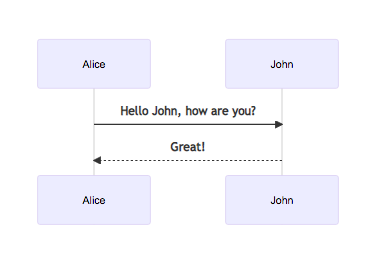
\includegraphics{img/mermaid.png}
\end{frame}

\hypertarget{mermaid-diagram-pdf-version}{%
\subsection{Mermaid diagram (PDF
version)}\label{mermaid-diagram-pdf-version}}

\begin{frame}[fragile]{Mermaid diagram (PDF version)}
Here a \texttt{.mermaid\ format=svg} hidden from slides in a ``notes''
section, but shows up in the README.

\note{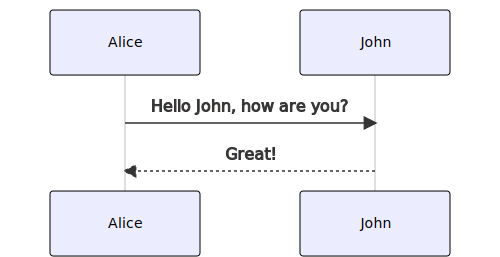
\includegraphics{img/mermaid.svg}}

The Makefile generates a PDF version that can be embedded\footnote<.->{https://tex.stackexchange.com/questions/2099/how-to-include-svg-diagrams-in-latex}
into the next slide with LaTeX's
\texttt{\textbackslash{}includegraphics}. So sometimes you have to
\texttt{make} twice.
\end{frame}

\hypertarget{mermaid-diagram-pdf-version-contd}{%
\subsection{Mermaid diagram (PDF version,
cont'd)}\label{mermaid-diagram-pdf-version-contd}}

\begin{frame}[fragile]{Mermaid diagram (PDF version, cont'd)}
Here's the \texttt{\textbackslash{}includegraphics} version, using the
PDF, which shows up in the PDF slides but not the README. Hat tip to
Jeromy Anglim.\footnote<.->{https://jeromyanglim.blogspot.com/2012/07/beamer-pandoc-markdown.html}

\centerline{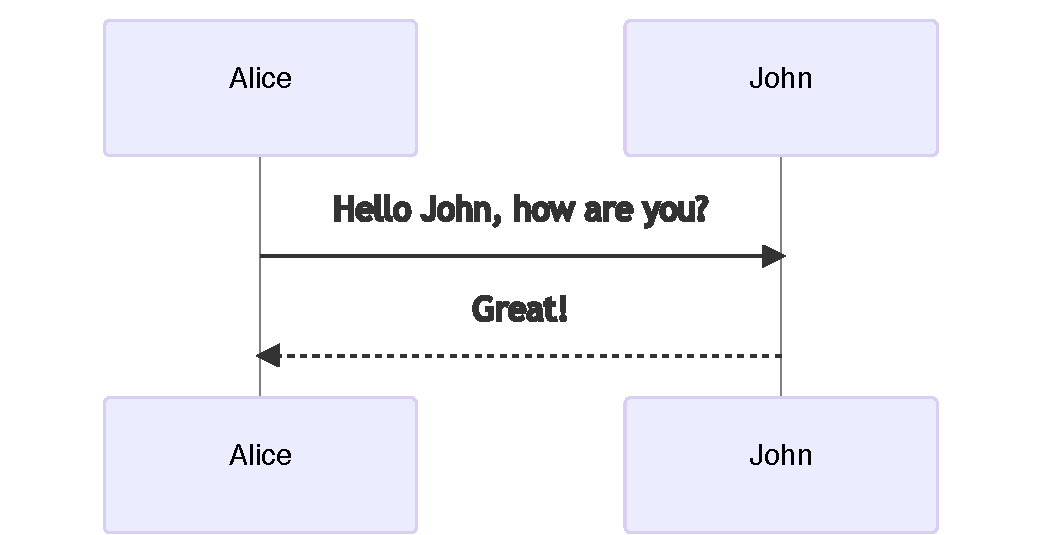
\includegraphics[width=3in]{img/mermaid.pdf}}
\end{frame}

\hypertarget{a-plain-slide-bottom-aligned}{%
\subsection{A plain slide,
bottom-aligned}\label{a-plain-slide-bottom-aligned}}

\begin{frame}[plain]{A plain slide, bottom-aligned}
Just a plain old slide.\footnote<.->{Do footnotes work? (not in GitHub,
  they don't)}
\end{frame}

\hypertarget{conclusion}{%
\subsection{Conclusion}\label{conclusion}}

\begin{frame}{Conclusion}
QED.
\end{frame}

\hypertarget{references-see-also}{%
\subsection{References / See Also}\label{references-see-also}}

\begin{frame}[fragile]{References / See Also}
\begin{itemize}
\tightlist
\item
  \url{https://garrettgman.github.io/rmarkdown/authoring_pandoc_markdown.html}

  \begin{itemize}
  \tightlist
  \item
    \href{https://garrettgman.github.io/rmarkdown/authoring_pandoc_markdown.html\#incremental_lists}{incremental
    lists}
  \item
    \href{https://garrettgman.github.io/rmarkdown/authoring_pandoc_markdown.html\#structuring_the_slide_show}{structuring
    the slide show}
  \end{itemize}
\item
  \url{https://github.com/jgm/pandoc/issues/5031}

  \begin{itemize}
  \tightlist
  \item
    basically,
    \texttt{\textbackslash{}framesubtitle\{The\ frame\textquotesingle{}s\ subtitle\}}
    is the only way
  \end{itemize}
\item
  \href{http://ctan.math.utah.edu/ctan/tex-archive/macros/latex/contrib/beamer/doc/beameruserguide.pdf}{beameruserguide.pdf}
\item
  \url{https://deic-web.uab.cat/~iblanes/beamer_gallery/}
\item
  \href{https://github.com/raghur/mermaid-filter}{mermaid-filter}

  \begin{itemize}
  \tightlist
  \item
    \href{https://github.com/github/markup/issues/270}{github/markup
    \#270} - GitHub doesn't support \texttt{data:} URIs in Markdown
  \item
    \href{https://tex.stackexchange.com/a/2107}{How to include SVG
    diagrams in LaTeX?}

    \begin{itemize}
    \tightlist
    \item
      I just ended up using librsvg's \texttt{svg2pdf} in the Makefile
    \end{itemize}
  \end{itemize}
\end{itemize}
\end{frame}

\end{document}
